\documentclass{article}

\usepackage[preprint]{neurips_2023}

\usepackage[utf8]{inputenc}
\usepackage[T1]{fontenc}
\usepackage{hyperref}
\usepackage{url}
\usepackage{booktabs}
\usepackage{amsfonts}
\usepackage{nicefrac}
\usepackage{microtype}
\usepackage{xcolor}
\usepackage{graphicx}
\usepackage{hyperref}


\title{Land-Cover Mapping with FLAIR-1: The Effects of Semantic Segmentation Model Architecture}


\author{
  Henry Feldhaus \\
  Department of Mechanical Engineering \\
  Carnegie Mellon University \\
  \texttt{hfeldhau@andrew.cmu.edu}
  \And
  Sanay Tralshawala \\
  Department of Mechanical Engineering \\
  Carnegie Mellon University \\
  \texttt{stralsha@andrew.cmu.edu}
}


\begin{document}


\maketitle


\begin{abstract}
% Write a brief summary (3--5 sentences) of your project: what problem you studied, what models you compared, and what you found. Delete all placeholder text in this template and replace it with your own writing before submitting.
Semantic segmentation of high-resolution aerial imagery enables automated land cover mapping at scale, supporting applications related to planning and monitoring. For this, we compare three architectures: ResNet34 U-Net, ConvNeXt-Tiny, DINOv3 ConvNeXt-Tiny on the FLAIR-1 dataset under RGB image data and a further ablation study into introducing Near Infrared and elevation data into the input features. The self-supervised learning DINOv3 ConvNeXt-Tiny model achieved the best test mIoU (0.491) and generalized most consistently, while supervised-pretrained ConvNeXt-Tiny improved validation performance but degraded on the test set, suggesting the benefit is specific to self-supervised pretraining rather than the ConvNeXt architecture alone. Five-channel inputs improved ConvNeXt-Tiny and DINOv3 but degraded ResNet34 U-Net, and conformal prediction analysis revealed that no model achieves 90\% marginal coverage, with minority classes failing severely across all configurations. However, using a larger dataset (over the implemented toy FLAIR-1 dataset), will be important to solidfy the conclusions made in this study.

\end{abstract}

% Page limits (including figures, excluding references and collaboration statement) are 3--4 pages for 1 person, 4--5 for 2, \textbf{5--6 for 3}, and 6--8 for 4 people. Please do not modify margins, font sizes, or spacing. Submit the final report as a PDF via Gradescope.


\section{Introduction}

% Address the following in this section:
% \begin{itemize}
%     \item What is the engineering or scientific context behind your dataset and prediction task?
%     \item How is the prediction or generation task motivated by the scientific domain?
%     \item What new capabilities are enabled if your model is successful?
% \end{itemize}

Semantic segmentation of remote-sensing imagery provides a comprehensive framework for understanding land-cover patterns, including urbanization, agricultural extent, and hydrology. By assigning a discrete class to every pixel, semantic segmentation enables the extraction of high-fidelity geo-spatial information that traditional image-level classification cannot provide. For city planners and environmental scientists, this level of detail is essential for converting raw aerial data into structured information for decision-making. However, manual interpretation of high-resolution images remains labor-intensive and difficult to scale across various terrains and acquisition conditions.

The FLAIR-1 dataset (\cite{ign2022flair1}) addresses the need for automated high-resolution mapping by providing a benchmark of 512×512 image patches across the French landscape. Each sample includes five input channels: red, green, blue, near-infrared (NIR), and elevation, and a semantically labeled pixel mask with 19 classes. To focus the experimental scope on major land-cover types and ensure manageable model comparisons, this study utilizes a simplified label space of six broad categories: built non-vegetated surfaces, bare non-vegetated surfaces, woody vegetation, cultivated land, herbaceous vegetation, and water. Given the dataset's inherent spatial and temporal domain variations, generalization remains a significant challenge, requiring models to resolve both fine spatial details, such as road boundaries, and broad visual patterns like vegetation distribution.

This study evaluates a ResNet34 U-Net baseline against modern ConvNeXt-based architectures, including a pretrained DINOv3 ConvNeXt variant. The objectives are to: (1) test whether modern convolutional backbones and self-supervised pretraining improve segmentation performance over pretrained encoder choices on a spatial segmentation task, (2) evaluate whether five-channel inputs using RGB, NIR, and elevation improve performance relative to RGB-only training, and (3) understand the confidence inherent in the resulting models.

Ultimately, advancing these segmentation techniques facilitates the production of faster, more consistent high-resolution maps, supporting critical applications in urban planning, disaster mitigation, and environmental assessment. Code and in-depth analysis can be found at: 
\url{https://github.com/sanay-tralshawala/DLE-Flair-Segmentation/}

\section{Methods}
For this analysis we choose three models to train and compare, all models are trained on the cross-entropy loss function based on the model's classification of each pixel.

\subsection{Baseline model: ResNet34 U-Net}

The baseline model is the ResNet34 U-Net, a choice consistent with the original benchmark established by \cite{ign2022flair1} for the  FLAIR-1 dataset. This architecture is particularly suited for high-resolution aerial imagery, as it combines deep learning powered feature extraction with the localization properties of the U-Net framework.

The model follows an encoder-decoder structure:
\begin{itemize}
    \item \textbf{Encoder (ResNet34)}: The backbone consists of 34 layers that use residuals to employ "skip connections" that learn identity mappings, mitigating the vanishing gradient problem. This allows the model to learn complex semantic features without losing the signal during backpropagation, as shown by \cite{he2016resnet}.
    \item \textbf{Decoder}: The decoder upsamples low-resolution feature maps back to the input spatial resolution and produces one logit map per semantic class.
    \item \textbf{Skip Connections}: Concatenations at layers between the encoder and decoder ensure features like edges and textures are preserved and assigned semantic meaning
\end{itemize}

ResNet34 U-Net has approximately 24.4 million parameters.

\subsection{Model Variant 1: ConvNeXt-tiny}
ConvNeXt \cite{liu2022convnet} introduces several architectural modernizations that differentiate it from ResNet's "standard" CNN architecture, namely, that it borrows design choices from Vision Transformers (ViT) introduced by \cite{DBLP:journals/corr/abs-2010-11929} while remaining purely convolutional.

ConvNeXt modernizes standard CNN design using larger convolution kernels, depthwise convolutions, inverted bottlenecks, GELU activations, and LayerNorm. These changes increase receptive field and improve feature extraction while retaining a convolutional inductive bias. For aerial imagery, this is useful because land-cover classes often depend on both local texture and broader spatial context.

In our experiments, the ConvNeXt-Tiny encoder is initialized from imported pretrained weights and fine-tuned for FLAIR-1 semantic segmentation. We implement ConvNeXt primarily because of its larger receptive field, which should allow the model to capture more context and understand larger-scale relationships, resulting in smaller Intersection over Union (IoU) losses. It also offers some ViT like performance without the requirement for massive training datasets, which we hope makes it easier to fine tune with limited data. 

ConvNeXt-tiny has 31.2 million parameters, representing a 28\% increase over ResNet34 U-Net.

\subsection{Model Variant 2: DINOv3-ConvNeXt-tiny}


The DINO (DIstillation with NO labels) family of models is a self-supervised learning framework for vision-based tasks, enabling learning from unlabelled internet-scale data. DINO models are also self-distilled using the student-teacher framework to learn smaller more efficient models from the large foundation models. Recently, Meta released DINOv3 ~\cite{simeoni2025dinov3}, a family of models pre-trained on 1.6 billion high-resolution images enabling high-fidelity feature extraction, making it uniquely suited for pixel-wise segmentation. The ConvNeXt-tiny architecture was one such model that pre-trained by Meta and released in this family. This model architecture and the corresponding weights were pulled from HuggingFace. In both ConvNeXt-tiny and DINOv3-ConvNeXt-tiny, a small decoder head was created to map the learned encodings into a pixel-wise classification system. This head is simply a 2-layer 2-dimensional convolution layer with ReLU normalization after the first layer. Each hidden layer has 256 nodes and network maps to a 6-node output for classification. Similarly, this model is left unfrozen and the entire model and backbone are trained or fine-tuned respectively

We implement this model primarily to compare the effectiveness an internet-scale dataset and a self-supervised backbone has on semantic segmentation. DINOv3-ConvNeXt-tiny has 29 million parameters, representing a 19\% increase over ResNet34 U-Net.

\subsection{Dataset and Preprocessing}
The full-scale FLAIR-1 training is computationally expensive (approximately 65 GB). This study uses the provided toy subset for controlled model comparison and as advised by Dr. Francis Ogoke. This limits the strength of claims about full-dataset performance, but it is sufficient for comparing relative behavior across architectures, input channels, and uncertainty-analysis methods under the same data constraints. The original train / validate / test subsets were restructured to an 80 / 10 / 10 split instead of the given 50 / 25 / 25; further, samples are assigned to maintain relative class frequencies in each subset.

We use the FLAIR-1 toy subset with six merged semantic classes: built non-vegetated surfaces, bare non-vegetated surfaces, woody vegetation, cultivated land, herbaceous vegetation, and water. All models are trained to predict a dense class mask from 512$\times$512 image patches. For RGB experiments, models receive the red, green, and blue channels. For five-channel experiments, models receive RGB, near-infrared, and elevation channels. The same train, validation, and test splits are used across models so that differences in performance can be attributed to model architecture and input-channel configuration rather than data variation.


\section{Results and Discussion}

% \textbf{Core evaluation (all groups).} Address the following:
% \begin{itemize}
%     \item Include at least one figure (for instance, plotting loss against training steps). Effective use of figures and tables is part of the grading criteria.
%     \item What metrics did you use to evaluate performance, and why are they appropriate for this task?
%     \item How does each model variant perform relative to the baseline? Report quantitative results.
%     \item Is your hypothesis from the Methods section supported by the data? Why or why not?
% \end{itemize}

We evaluate model performance primarily using the mean Intersection over Union (mIoU), mean Dice score, and pixel accuracy. mIoU is our primary metric because this is multi-class segmentation task: it measures the overlap between the predicted and ground-truth regions for each class, then averages across classes. We use the mean to ensure a generalized metric when class frequencies are imbalanced, as in this dataset. Dice score is a complementary overlap-based measure that is also common in segmentation tasks, with a lower threshold for small regions. Pixel accuracy is included as a sanity check, but is considered a secondary metric because it can mask minor classes' poor performance.

% \begin{figure}[h]
%   \centering
%   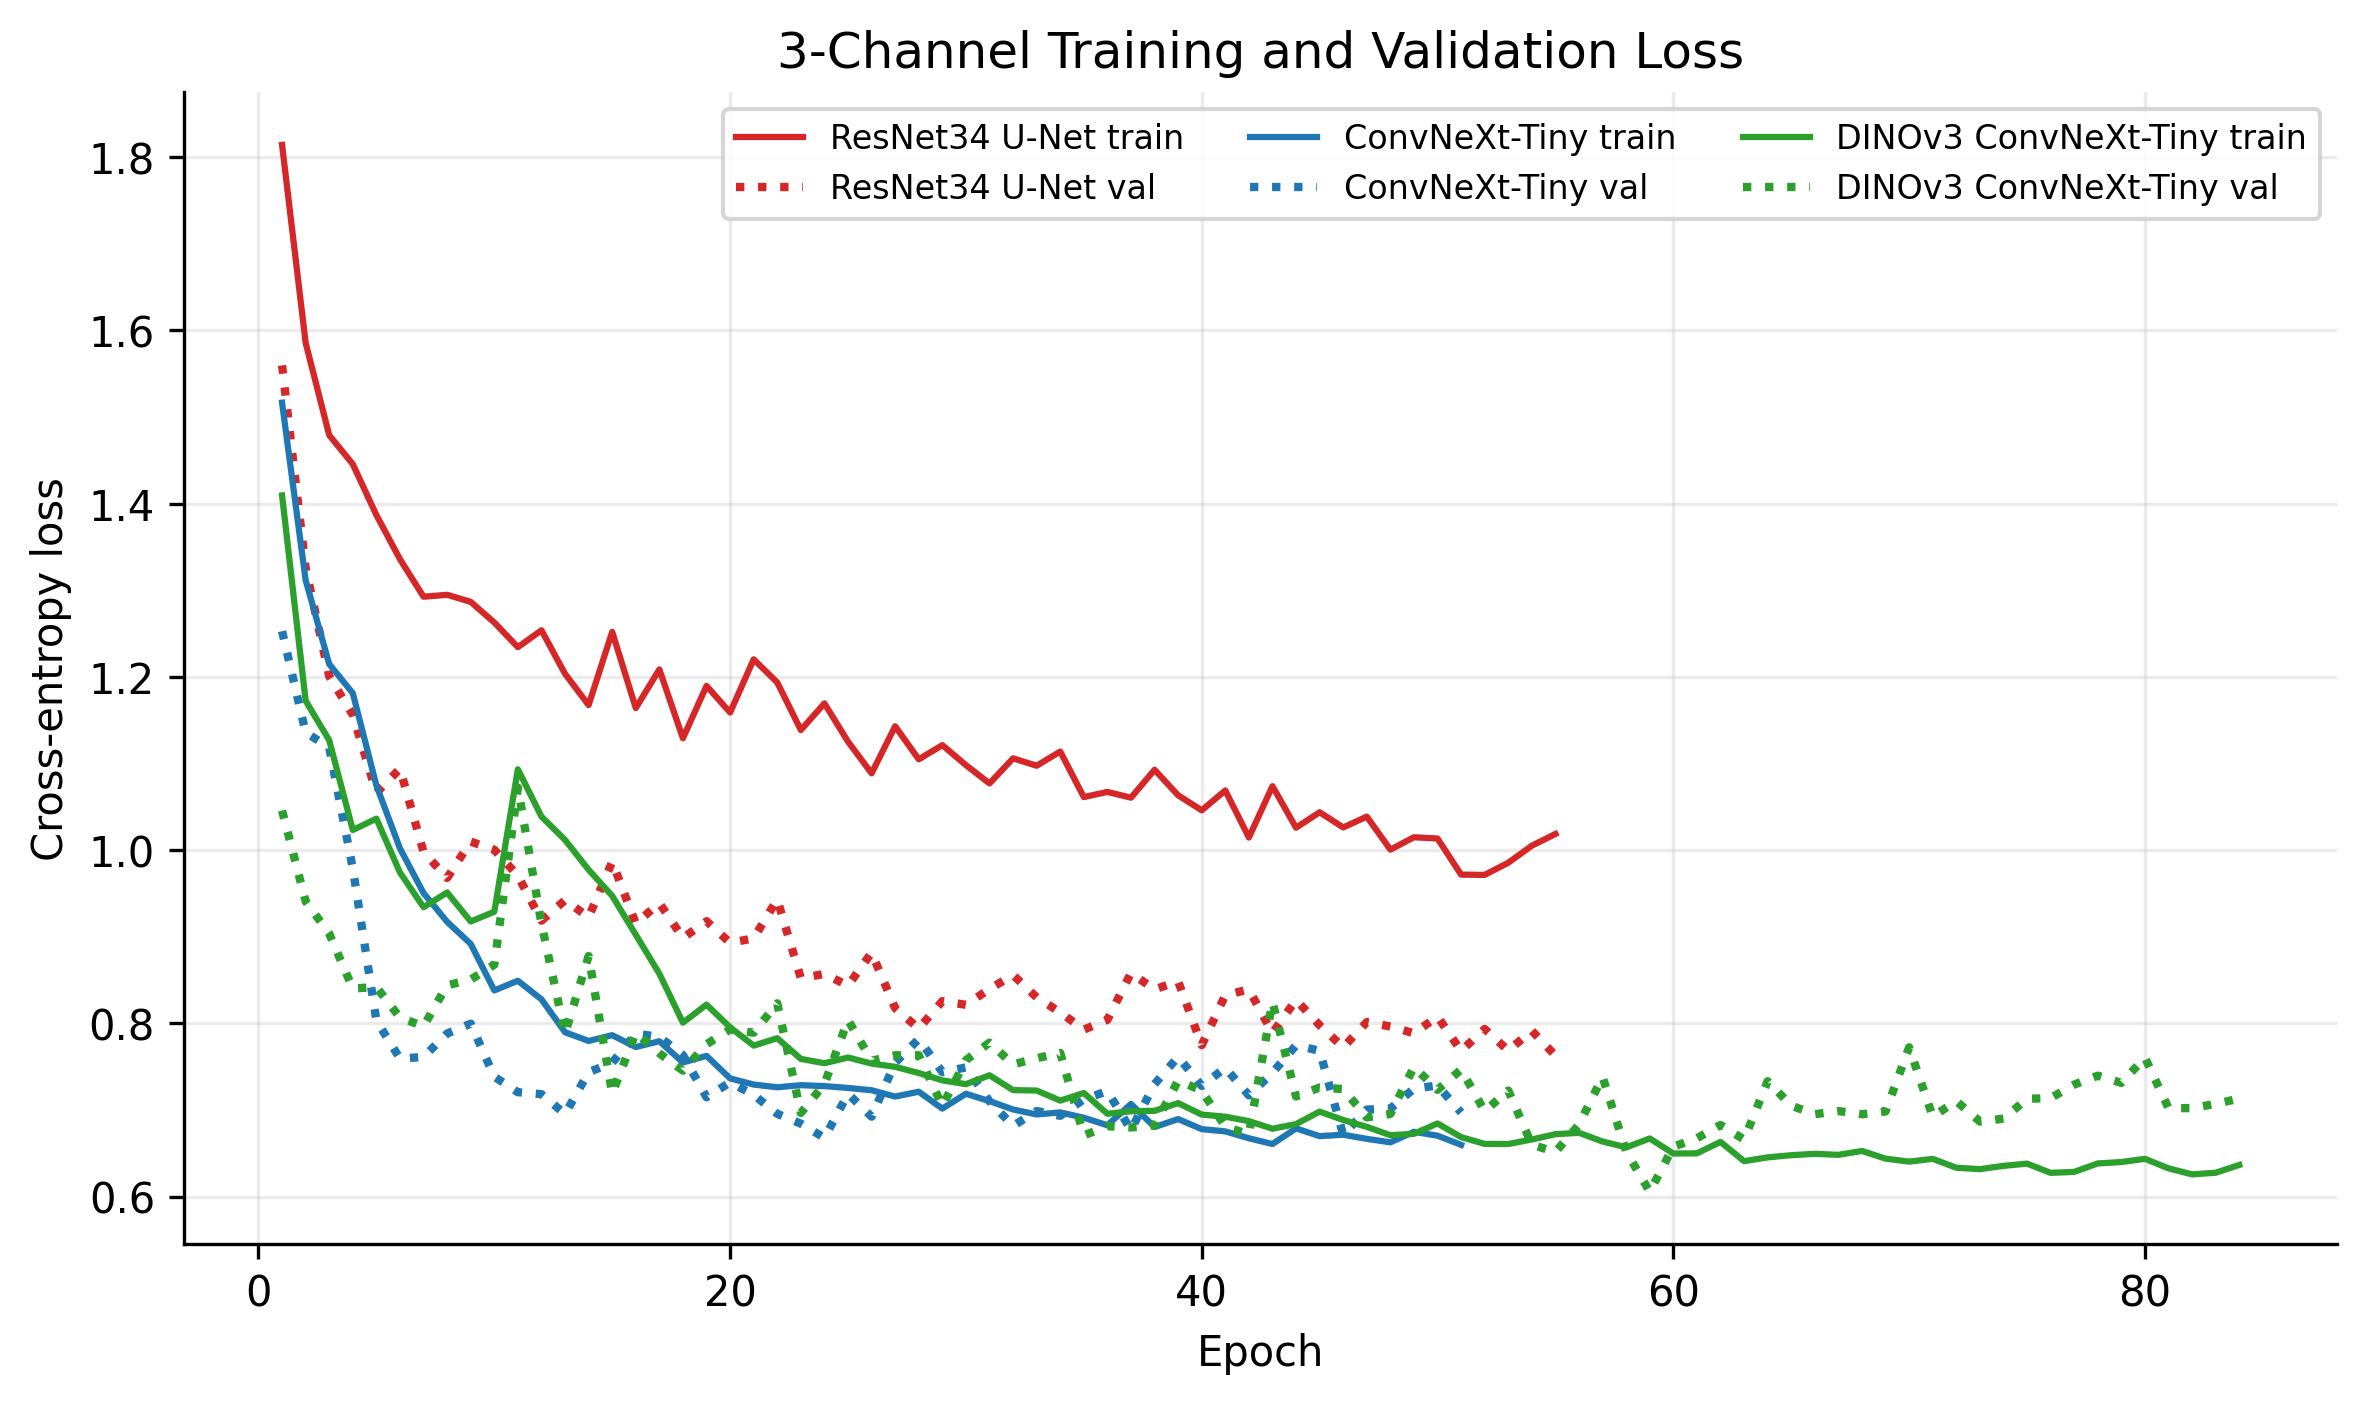
\includegraphics[width=0.9\linewidth]{figures/3ch_train_val_loss.png}
%   \caption{Training and validation cross-entropy losses by model. Implemented early-stopping (metric: validation mIoU, patience: 25 epochs) explains variable length of loss curves; "best" checkpoints are recorded according to validation mIoU.}
%   \label{fig:losses}
% \end{figure}

\begin{figure}[h]
  \centering

  \begin{minipage}{0.49\linewidth}
    \centering
    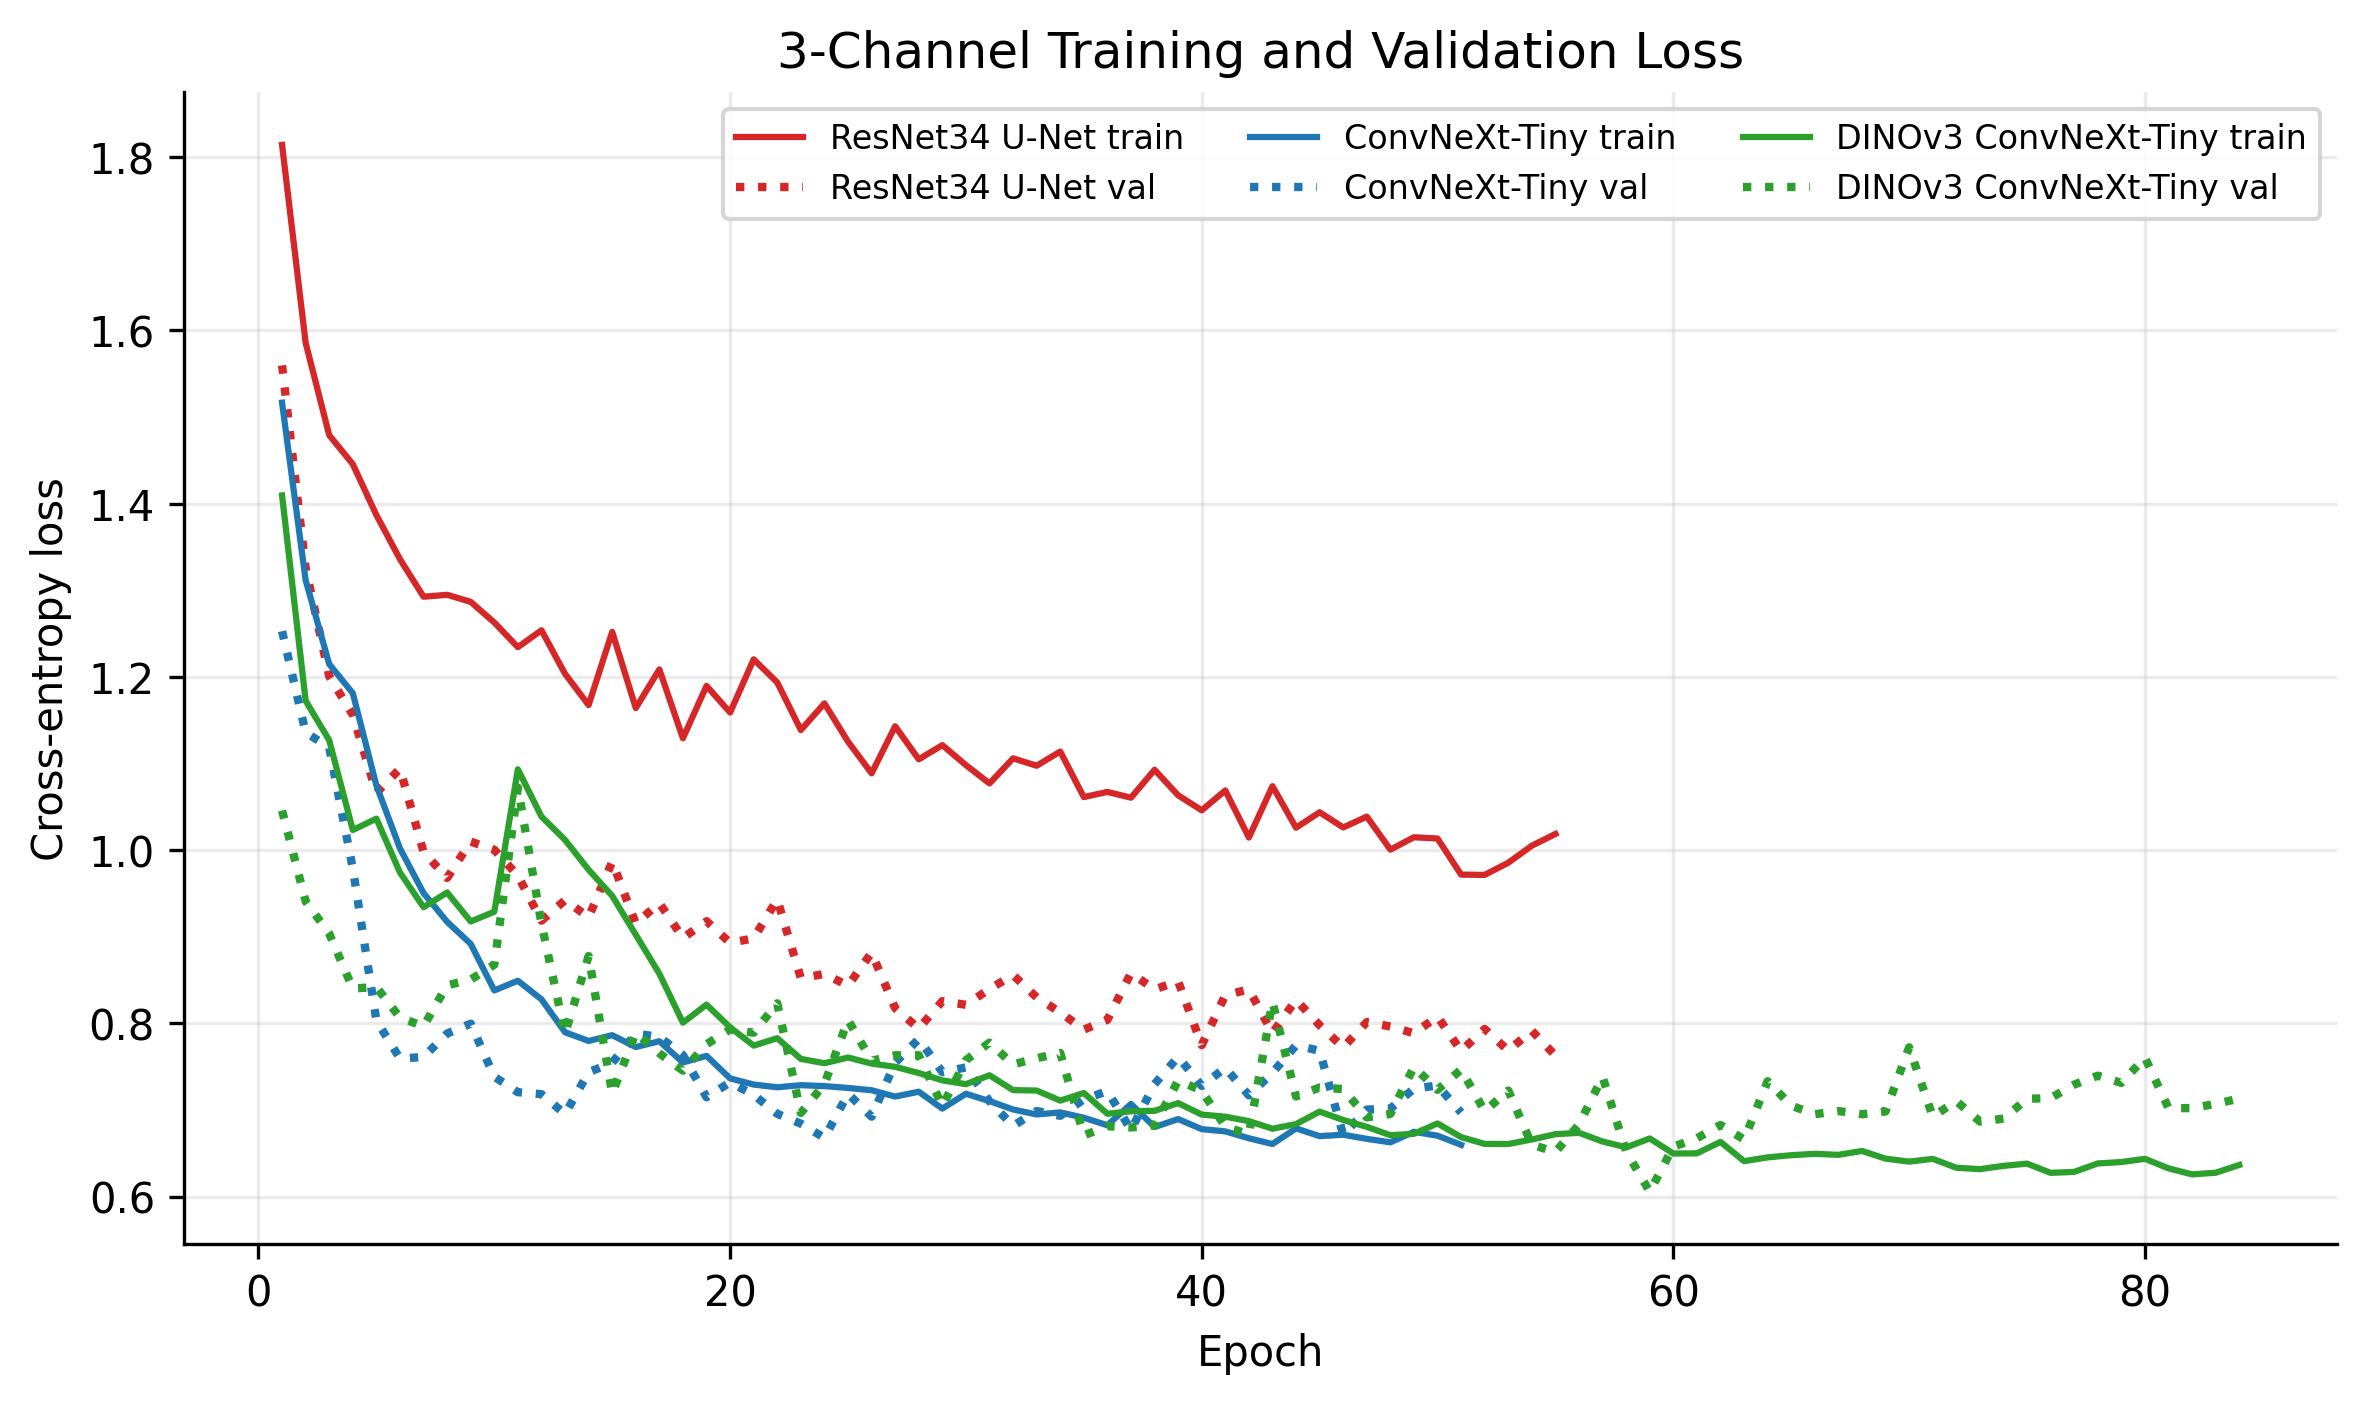
\includegraphics[width=\linewidth]{figures/3ch_train_val_loss.png}
  \end{minipage}
  \hfill
  \begin{minipage}{0.49\linewidth}
    \centering
    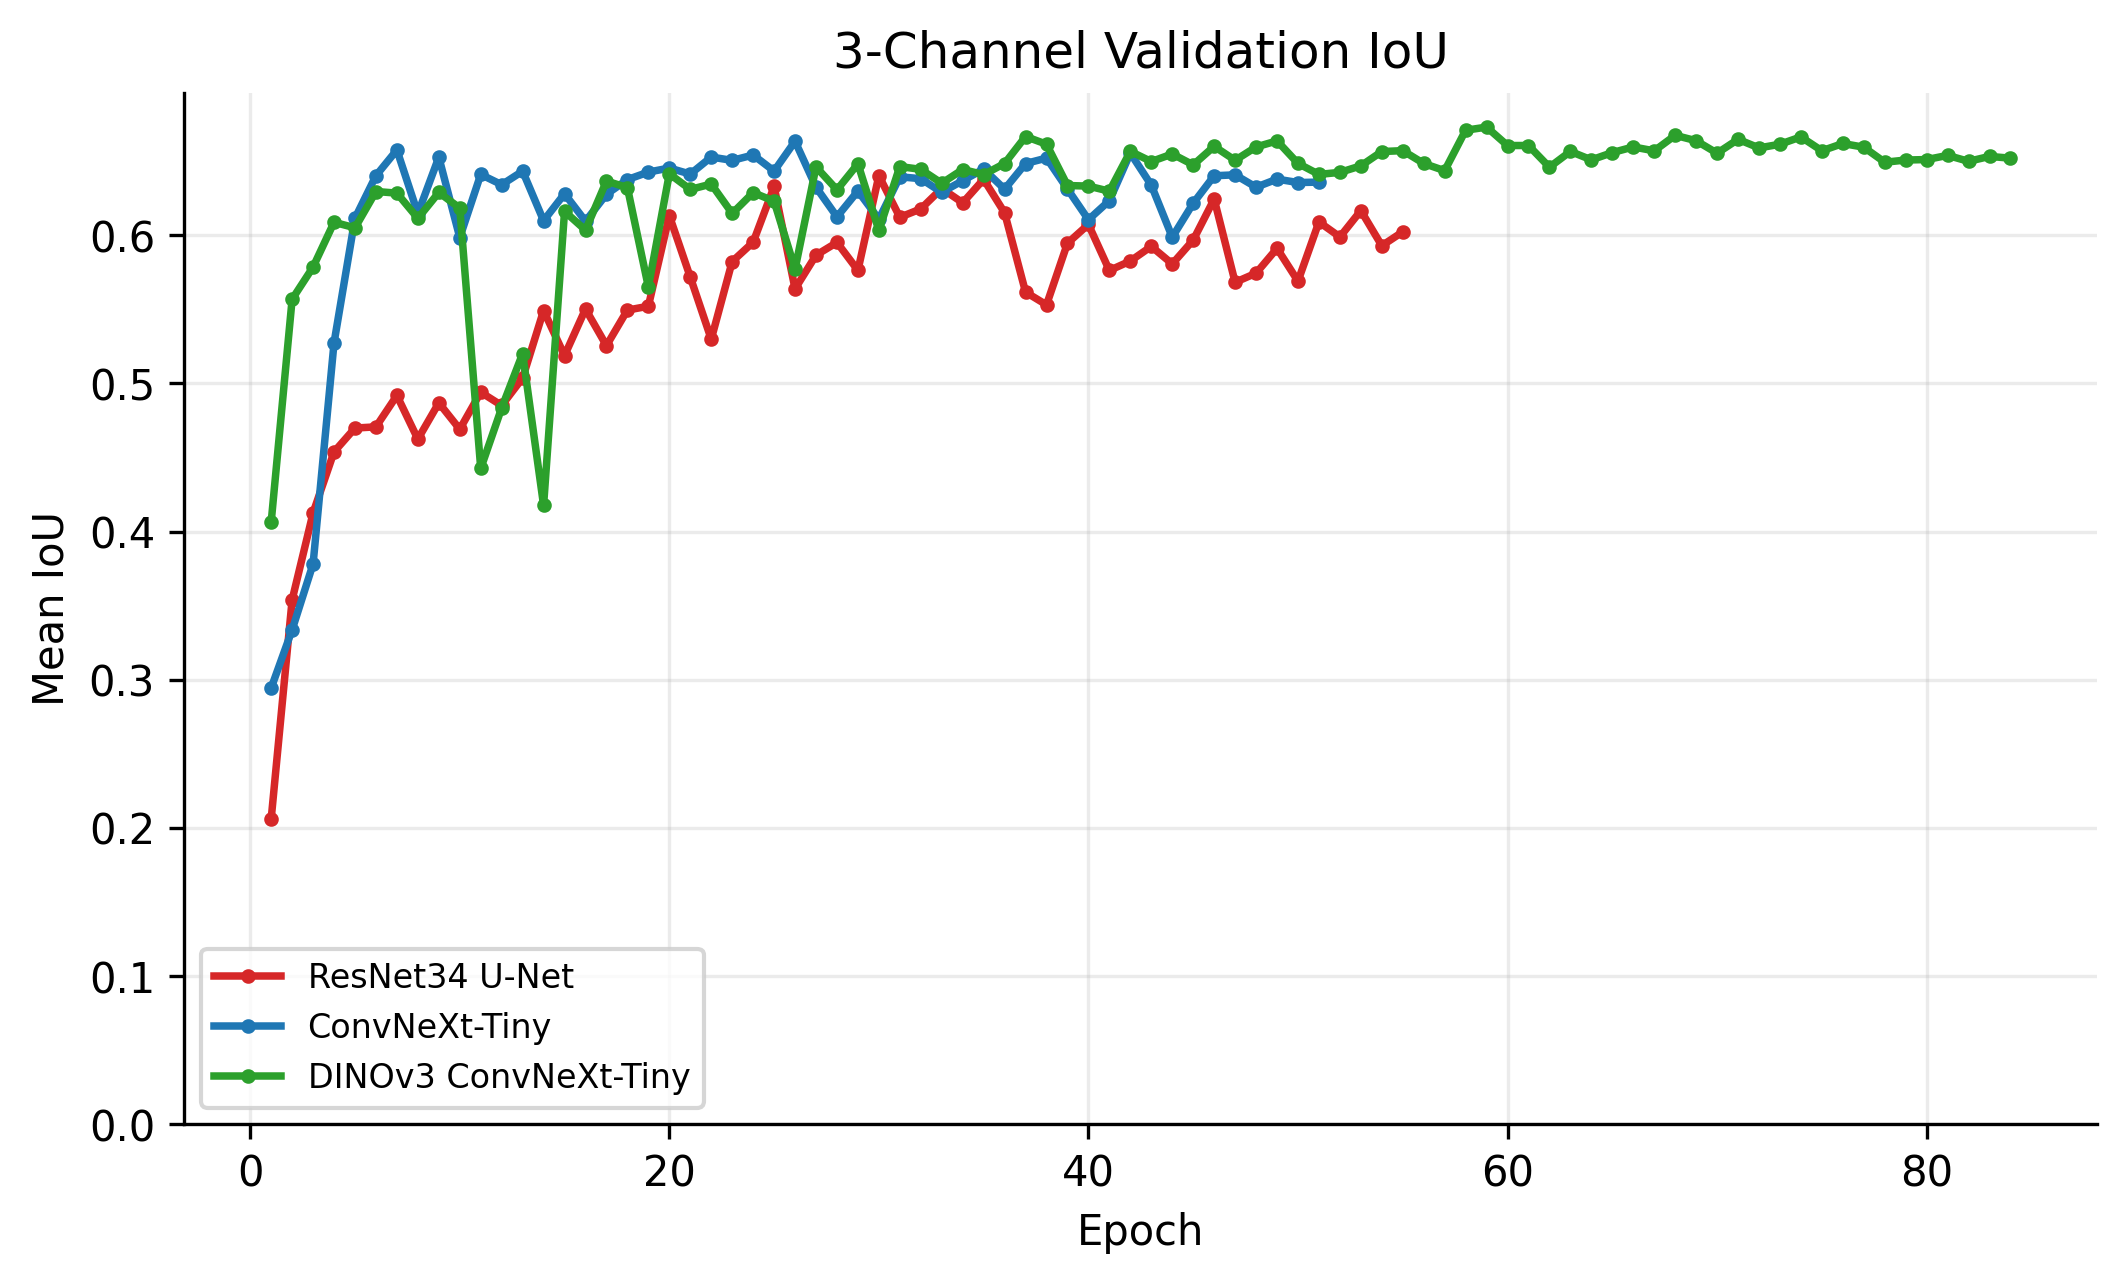
\includegraphics[width=\linewidth]{figures/3ch_val_iou.png}
  \end{minipage}

  \caption{(a) Training and validation cross-entropy losses by model. Implemented early-stopping \textit{(metric: val. mIoU, patience: 25 epochs)} explains variable length of loss curves; ``best'' checkpoints are recorded according to validation mIoU. (b) mIoU by model for the same runs.}
  \label{fig:losses}
\end{figure}

Using ResNet34 U-Net as the baseline, both ConvNeXt variants achieved higher validation mIoU, but their test behavior differed. DINOv3 ConvNeXt-Tiny achieved the strongest test performance, improving test mIoU from 0.460 to 0.478 and producing the highest mean Dice score. In contrast, ConvNeXt-Tiny improved validation mIoU but underperformed the baseline on the held-out test set. This suggests that the DINOv3-pretrained ConvNeXt encoder provided a modest generalization benefit over the supervised-pretrained ConvNeXt encoder under the limited-data setting. The gap between validation and test mIoU across all models also indicates limited generalization from the toy validation split to the test split, likely due to small sample size in the toy dataset and terrain variability.

\begin{table}[h]
  \caption{Validation and test performance for semantic segmentation models.}
  \label{tab:model_performance}
  \centering
  \begin{tabular}{lccccc}
    \toprule
    Model & Val mIoU & \textbf{Test mIoU} & Test Pixel Acc. & Test Mean Dice \\
    \midrule
    ResNet34 U-Net & 0.639 & \textbf{0.460} & 0.729 & 0.589 \\
    ConvNeXt-Tiny & 0.665 & \textbf{0.447} & 0.693 & 0.571 \\
    DINOv3 ConvNeXt-Tiny & 0.668 & \textbf{0.478} & 0.725 & 0.604 \\
    \bottomrule
  \end{tabular}
\end{table}

Overall, the architecture hypothesis is only partially supported. DINOv3 ConvNeXt-Tiny achieved the best test mIoU and mean Dice, but the gain over the ResNet34 U-Net baseline was modest. The supervised-pretrained ConvNeXt-Tiny model improved validation mIoU but did not improve test performance, suggesting that the DINOv3 self-supervised pretraining strategy provided better generalization than the supervised-pretrained ConvNeXt encoder. However, because all models used imported pretrained weights, these results should be interpreted as a comparison of backbone architecture and pretraining source, not as a comparison against training from scratch.

\subsection{Additional Analysis 1: Channel Ablation}
The original Flair-1 dataset includes 5-channel samples, while the primary experiments in this study focus on the first three color channels. Our pre-trained backbones were only trained on 3-channel input data, so an additional 2 channels of weights are assigned. To test if the extra channels (IR, elevation) were useful, we trained matching 5-channel models from the pretrained RGB backbones, adapted to accept an additional two channels. We compared their full 5-channel test performance against the corresponding 3-channel models; furthermore, we ablated the extra channels at inference time by zeroing channels 4 and 5, leaving the remaining weights otherwise unchanged. A summary of results is shown in Table~\ref{tab:channel_ablation}.

\begin{table}[h]
  \caption{5-channel training and channel ablation results on the test split.}
  \label{tab:channel_ablation}
  \centering
  \begin{tabular}{lccccc}
    \toprule
    Model & 3ch mIoU & 5ch mIoU & $\Delta$ vs. 3ch & Zeroed 4+5 mIoU \\    
    \midrule
    ResNet34 U-Net & 0.460 & 0.436 & -0.024 & 0.262 \\
    ConvNeXt-Tiny & 0.447 & 0.484 & +0.037 & 0.450 \\
    DINOv3 ConvNeXt-Tiny & 0.478 & 0.491 & +0.013 & 0.498 \\
    \bottomrule
  \end{tabular}
\end{table}

Fine tuning with five channels improved the test mIoU for ConvNeXt-tiny and the DiINOv3 ConvNeXt variant, but degraded ResNet34 U-net. ConvNeXt-Tiny gained $+0.037$ mIoU over its 3-channel version and dropped by $0.034$ mIoU when channels 4 and 5 were removed, suggesting that it learned to use the added inputs. DINOv3 improved modestly over its 3-channel version, but its ablated score was slightly higher than its full 5-channel score, so the gain is not clearly attributable to the extra channels. ResNet34 U-Net relied heavily on the extra channels under ablation, but its full 5-channel performance was still below the 3-channel baseline, suggesting less robust use of the additional inputs. For more in depth results refer to the \verb|07_channel_comparison.ipynb| notebook.

\subsection{Additional Analysis 2: Conformal Prediction}

To further investigate the learning capabilities of the models and the nuances related to our model's performance, we performed a Conformal Prediction \cite{DBLP:journals/corr/abs-2107-07511} study to understand the size of the prediction set required for each pixel to obtain a specified confidence score. More specifically, we to understand the required set size of predicted class labels for each pixel classification to include the ground truth label 90\% of the time. This study sheds light into the confidence and uncertainty in a model and understand whether empirical coverage is met for each class. The validation dataset was used as the calibration set. Though the models chosen for analysis was a result of the model's performance in the validation set, to maintain i.i.d and exchangability assumptions, we consider this model as a result of converged train loss, which generally holds true. All six models in the channel ablation study were used for analysis. In a classification sense, the analysis determines the softmax threshold to be included in a solution set. Even though we are investigating semantic segmentation, this process focuses on the per pixel classification as this analysis focuses on the pixel-level uncertainty of the semantic segmentation model. Thus, table ~\ref{tab:conformal prediction} shows the results of this study analyzing the empirical coverage per class and the overall coverage for each model. 

\begin{table}[h]
  \caption{Conformal Prediction Empirical coverage w.r.t $90\%$ confidence score}
  \label{tab:conformal prediction}
  \centering
  \resizebox{\textwidth}{!}{
  \begin{tabular}{lcccccc}
    \toprule
    Class & 3ch ResNet34 & 5ch ResNet34 & 3ch ConvNeXt & 5ch ConvNeXt & 3ch DINOv3 & 5ch DINOv3  \\    
    \midrule
    Built (Non-vegetated) & 97.10 & 97.74 & 93.11 & 97.51 & 97.81 & 98.07\\ 
    Bare (Non-vegetated) & 10.00 & 10.91 & 6.03 & 34.45 & 23.26 & 48.69\\
    Woody Vegetation & 97.27 & 91.61 & 88.06 & 88.35 & 90.07 & 95.92\\
    Agriculture & 83.07 & 96.92 & 83.13 & 82.33 & 83.86 & 95.55\\
    Herbaceous vegetation & 71.49 & 74.07 & 70.90 & 82.72 & 64.00 & 53.30\\
    Water & 45.90 & 47.62 & 57.19 & 51.00 & 81.27 & 95.23\\
    Ovr Model & 84.01 & 85.24 & 80.84 & 84.99 & 84.27 & 87.67\\
    Pixel avg set size & 1.444 & 1.444 & 1.377 & 1.523 & 1.423 & 1.450\\
    \bottomrule
  \end{tabular}
  }
\end{table}

By class, the models performed quite poorly related to the Bare (Non-vegetated) class ($<50\%$) and to a lesser extent the Herbaceous vegetation. Moreover, the water class performed quite well only for the DINOv3 based models and the Built (Non-vegetated) class performed exceptionally well. For Woody Vegetation and Agriculture, across the board the results stayed around the 90\% coverage requirement though some models aired below this line, indicating that we cannot guarantee the desired coverage for the model. This extents to the overall model, where there is not a single model that meets the desired confidence - though the DINOv3 model with 5 channels noticeably produced a 3\% increase in coverage. Between 3 channels and 5 channels, there is not a noticeable difference in coverage though minor increases in coverage can be observed for most of the models when increasing to 5 channels. Though the average pixel set size is less than 2, which indicates minimal uncertainty, this is skewed by exceptionally well performing classes for a specific model. Further, it can be noticed that the prediction set size for an image increases with incorrect predictions as well as for classes with a low amount of data. For more in depth results refer to the \verb|05_conformal_prediction.ipynb| notebook.

\begin{figure}
    \centering
    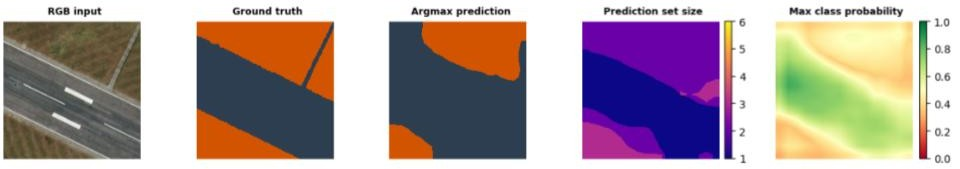
\includegraphics[width=1\linewidth]{figures/Testimage results.jpg}
    \caption{The RGB image, segmented ground truth, predicted image and calibrated prediction set on a test case}
    \label{fig:testimage results}
\end{figure}

\section{Conclusion}

This study compared the ResNet34 U-Net, ConvNeXt-tiny, models DINOv3 ConvNeXt-tiny on the FLAIR-1 toy dataset under three and five channel inputs and with conformal prediction to analyze possible coverage guarantees and characterize per-class uncertainty. The hypothesis that more modern architectures and a self-supervised pretrained model would improve segmentation was partially supported. The DINOv3 model produced the best test mIOU, though by a minimal margin, in both 3 channel and 5 channel configurations. This indicates that internet-scale pretraining could be effective and provide consistent generalization. Supervised-pretrained ConvNeXt-Tiny improved validation mIoU but degraded on the test set, suggesting the benefit is specific to the DINOv3 pretraining strategy rather than the ConvNeXt architecture alone.

Similarly, the study introducing near infrared and elevation data to the original RGB channels is not noticeably clear. ConvNeXt-tiny produced the highest increase when increasing channels by an increase of 0.037 mIoU score. The DINOv3 model performed well with a modest improvement when increasing channels. On the other hand, ResNet-34 U-Net degraded, indicating less robust weight adaption across both models. Conformal Prediction revealed that no model reliably met the 90\% coverage guarantee. Bare (Non-vegetated) failed severely across all six configurations, consistent with its low training size (4.7\% of dataset). The small average prediction set sizes (1.38–1.52) is misleading — it is driven by high-confidence majority classes and masks critical under-coverage for minority classes. Such a general trend can be noticed between data size per class and the confidence the class exhibits. 

This unveils a bigger gap in our analysis. The toy dataset is relatively small compared to the full dataset and for the deep architectures used in this report. The immediate next step, if given proper compute, time, and relaxed constraints, would be to train on the full FLAIR-1 dataset and to include a fully independent calibration set for confidence analysis. With more data, our conclusions would be more robust and reliable. Further, optimizing the use of multiple channels should be investigated - specifically if a certain configuration of features will produce better results for satellite imagery, not necessarily just the RGB channels or RGB-NIR-Elevation channels.

\section*{Collaboration Statement}

A W\&B project report dashboard, contained all training runs for this investigation, is available in the
\href{https://api.wandb.ai/links/flair-segmentation-dle/xepqbnmw}{Weights \& Biases report} (hyperlinked).

\subsection{Henry's Contributions}
Henry's primary responsibilities included: (1) conducting exploratory data analysis (EDA), collapsing the original classes, and reassigning the train, validation, and test splits; (2) writing the main training loop used across the models; (3) iterating on ConvNeXt-Tiny training experiments; (4) evaluating the final models on the test set and extracting core test metrics; (5) conducting the additional 3-channel vs. 5-channel input ablation study; and (6) writing the introduction, ResNet34 U-Net overview, ConvNeXt overview, portions of the results section, and the ablation study section of the report. He also implemented Weights \& Biases (W\&B) logging for the project.

Henry used GitHub Copilot as an implementation and debugging aid rather than as a replacement for project design or analysis. His general workflow was to first define the intended architecture through pseudocode comments, stub functions, and prior examples from class, then write and adapt the implementation based on his own understanding of the pipeline. When errors arose, he used Copilot to help reason through debugging steps, improve robustness, and suggest refactors such as splitting larger functions into smaller helper and driver functions. Copilot was primarily used to accelerate implementation details, error handling, and code organization, while Henry remained responsible for the pipeline structure, experiment design, model training decisions, evaluation, and interpretation of results.
\subsection{Sanay's Contributions}

Sanay's primary responsibilities included: (1) generating the appropriate model architectures and creating a model loaders for each model, (2) producing a dataloader to consistently read and process the data, (3) iterate on DINOv3 ConvNeXt-Tiny training experiments, (4) conducting the calibration study and the conformal prediction analysis and evaluation, and (5) writing the Abstract, DINOv3 ConvNeXt-Tiny overview, portions of the results section, and the calibration study section of the report. Sanay also organized and wrote the \verb|README.md| for the related code base. 

Sanay used Gemini coding assistance in Google Colab for implementation and debugging tool. Once a code base/file was established, an attempt to implement the code or to test the code was made, the AI agent was used to debugging assistance patch up the code, this mainly was for Colab patch work such as basic Object-Orientated programming assistance with Jupyter Notebook, and implementing Colab features such as Colab secrets and using git control via Google Drive. Specifically for Conformal Prediction, Claude was used as an idea sounding board, where the core idea was proposed and with the help of the LLM was refined into a concrete and plausible idea that was independently generated and debugged via the LLM. The work produced by Sanay, including the general logic and ideation is fundamentally his own with generative AI used to help bring these ideas to fruition.




\bibliographystyle{unsrtnat}
\bibliography{refs}


\end{document}

% Sample figure (uncomment and replace with your own):
% \begin{figure}[h]
%   \centering
%   \includegraphics[width=0.8\linewidth]{your_figure.pdf}
%   \caption{Description of your figure.}
%   \label{fig:example}
% \end{figure}

% Sample table (uncomment and replace with your own):
% \begin{table}[h]
%   \caption{Description of your table.}
%   \label{tab:example}
%   \centering
%   \begin{tabular}{lcc}
%     \toprule
%     Model & RMSE & $R^2$ \\
%     \midrule
%     Baseline (PointNet) & 0.142 & 0.85 \\
%     Variant (PointNet++) & 0.118 & 0.90 \\
%     \bottomrule
%   \end{tabular}
% \end{table}